% The hook, for a full-bleed UMB-blue title-style slide. Drawn white and accent only, with no
% background fill, so it sits on the blue slide. The message arrives at 16:40, the doors open at
% 17:00: a 20-minute wedge on the clock. Facts from the recorded development run.
\documentclass[border=3pt]{standalone}
% Shared style of every Plan B figure (the deck, the poster and the documentation).
% Type is near-black and grey on white. UMB blue is the brand and the system. One warm accent
% marks tension only (the incoming message, the clock). Green marks only an accepted receipt or
% a met run. Square corners, thin rules, no shadows, no gradients.
\usepackage[T1]{fontenc}
\usepackage[scaled]{helvet}
\renewcommand{\familydefault}{\sfdefault}
\usepackage{tikz}
\usepackage{pgfplots}
\pgfplotsset{compat=1.18}
\usepackage{fontawesome5}
\hyphenpenalty=10000
\exhyphenpenalty=10000
\usetikzlibrary{arrows.meta,positioning,calc,fit,backgrounds}

% Colours
\definecolor{primary}{HTML}{08457E}   % UMB blue: the system, Plan B's own policy
\definecolor{primarysoft}{HTML}{E7EEF5}
\definecolor{accent}{HTML}{FF791F}    % tension only: the message, the gap, the one missed run
\definecolor{accentsoft}{HTML}{FFEBDC}
\definecolor{umbblue}{HTML}{005A8B}   % UMB blue: the three idea marks and structure
\definecolor{navy}{HTML}{132245}      % title bands, the receipt, the dark close
\definecolor{ground}{HTML}{EEF2F6}    % the light blue-grey ground behind white cards
\definecolor{ok}{HTML}{2E7D32}        % an accepted receipt, a met run
\definecolor{oksoft}{HTML}{E5F1E6}
\definecolor{ink}{HTML}{1F1F1F}
\definecolor{muted}{HTML}{6B6B6B}
\definecolor{quiet}{HTML}{9A9A9A}     % other policies, context
\definecolor{rulegrey}{HTML}{C4C4C4}
\definecolor{gridgrey}{HTML}{E4E4E4}
\definecolor{faint}{HTML}{F4F4F4}

\tikzset{
  >={Stealth[length=2.4mm,width=1.8mm]},
  every picture/.style={line cap=butt, line join=miter},
  % text styles
  hd/.style={font=\bfseries, text=ink, align=left},
  sub/.style={text=muted, align=left},
  % shapes: square or 1 pt corners, thin rules
  card/.style={draw=rulegrey, line width=0.5pt, fill=white, rounded corners=1pt, inner sep=5pt, align=left, text=ink},
  sys/.style={draw=primary, line width=0.8pt, fill=white, rounded corners=1pt, inner sep=5pt, align=center, text=ink},
  sysfill/.style={draw=primary, line width=0.8pt, fill=primary, rounded corners=1pt, inner sep=5pt, align=center, text=white},
  warm/.style={draw=accent, line width=0.8pt, fill=accentsoft, rounded corners=1pt, inner sep=5pt, align=left, text=ink},
  receipt/.style={draw=ok, line width=0.8pt, fill=oksoft, rounded corners=1pt, inner sep=5pt, align=left, text=ink},
  planned/.style={draw=muted, line width=0.6pt, dash pattern=on 3pt off 2pt, fill=white, rounded corners=1pt, inner sep=5pt, align=left, text=muted},
  % connectors
  link/.style={->, draw=muted, line width=0.6pt},
  syslink/.style={->, draw=primary, line width=0.9pt},
  oklink/.style={->, draw=ok, line width=0.9pt},
  warmlink/.style={->, draw=accent, line width=0.9pt},
  nextlink/.style={->, draw=muted, line width=0.6pt, dash pattern=on 3pt off 2pt},
}

% Charts: a real axis, few light gridlines, no frame on the top and right.
\pgfplotsset{
  planb/.style={
    axis line style={draw=muted, line width=0.5pt},
    tick style={draw=muted, line width=0.5pt},
    major tick length=3pt,
    tick label style={text=ink, /pgf/number format/assume math mode=true},
    label style={text=ink},
    title style={font=\bfseries, text=ink},
    grid style={draw=gridgrey, line width=0.4pt},
    every axis plot/.append style={line width=0.6pt},
    legend style={draw=none, fill=none, text=ink},
    legend cell align=left,
  },
}

% The three idea marks, the same in the deck, the poster and the report.
% 1 Check the fact (a magnifier), 2 Pick only what fits (a funnel that keeps what fits),
% 3 Leave a receipt (a receipt slip). Always in UMB blue unless the panel is navy.
\providecommand{\markcheck}{\faSearch}
\providecommand{\markfits}{\faFilter}
\providecommand{\markreceipt}{\faReceipt}
% The three points of "Why Plan B": safer shows the three marks together, more flexible a laptop,
% more personal a set of sliders.
\providecommand{\marksafer}{\faSearch\,\faFilter\,\faReceipt}
\providecommand{\markflexible}{\faLaptop}
\providecommand{\markpersonal}{\faSlidersH}

\begin{document}
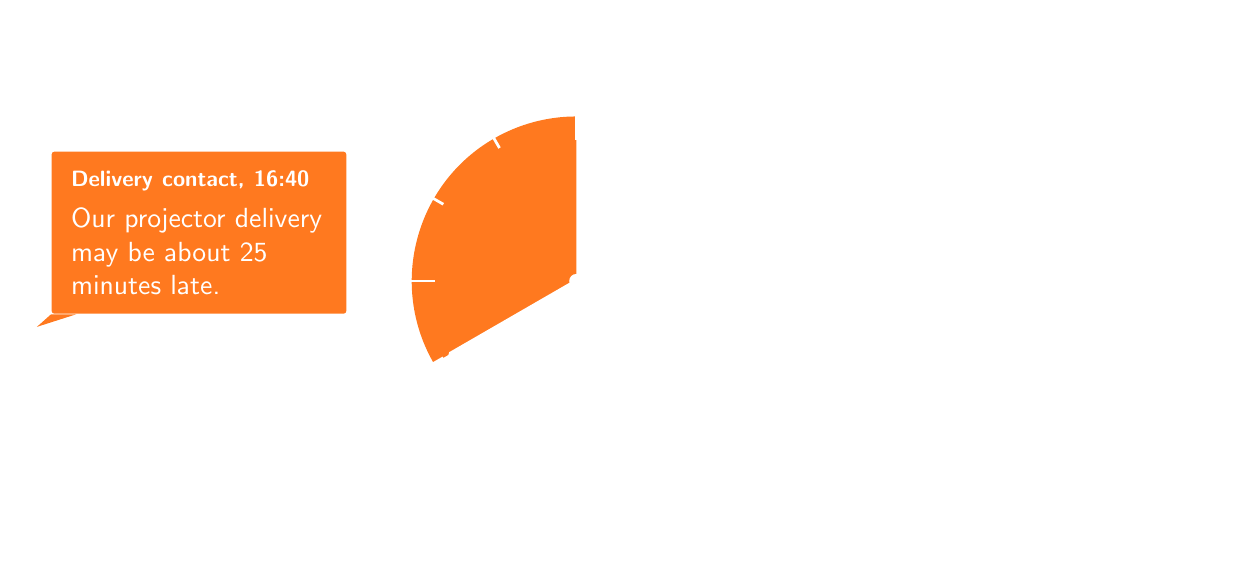
\begin{tikzpicture}[x=1cm, y=1cm, line join=round]
  % ---------------------------------------------------------------- the phone
  \def\pw{4.3}   % phone width
  \def\ph{6.4}   % phone height
  \draw[white, line width=1pt, rounded corners=0.5cm] (0,0) rectangle (\pw,\ph);
  \draw[white, line width=1pt, line cap=round] (\pw/2-0.4,\ph-0.32) -- (\pw/2+0.4,\ph-0.32);   % speaker
  \draw[white, line width=1pt, line cap=round] (\pw/2-0.55,0.28) -- (\pw/2+0.55,0.28);          % home bar
  % the incoming message
  \node[anchor=north west, fill=accent, text=white, inner sep=7pt, text width=3.25cm, align=left,
        font=\normalsize, rounded corners=1pt] (msg) at (0.28,\ph-1.55)
    {{\footnotesize\bfseries Delivery contact, 16:40}\\[3pt]
     Our projector delivery\\ may be about 25\\ minutes late.};
  \fill[accent] ($(msg.south west)+(0,0.0)$) -- ($(msg.south west)+(-0.18,-0.16)$) -- ($(msg.south west)+(0.32,0)$) -- cycle;

  % ---------------------------------------------------------------- the clock at 16:40
  \def\cx{6.95}
  \def\cy{3.2}
  \def\r{2.15}
  \begin{scope}[shift={(\cx,\cy)}]
    % the 20 minutes from 16:40 to 17:00
    \fill[accent] (0,0) -- (210:\r-0.06) arc[start angle=210, end angle=90, radius=\r-0.06] -- cycle;
    \draw[white, line width=1pt] (0,0) circle (\r);
    \foreach \h in {0,...,11}{
      \pgfmathsetmacro{\len}{mod(\h,3)==0 ? 0.36 : 0.2}
      \draw[white, line width=1pt] (90-\h*30:\r) -- (90-\h*30:\r-\len);
    }
    % hands: hour at 4:40, minute at 40
    \draw[white, line width=2.2pt, line cap=round] (0,0) -- (-50:1.15);
    \draw[white, line width=1.4pt, line cap=round] (0,0) -- (210:1.85);
    \fill[white] (0,0) circle (0.09);
  \end{scope}

  % ---------------------------------------------------------------- the words
  \node[anchor=west, text=white, align=left, inner sep=0pt, font=\fontsize{24}{27}\selectfont\bfseries]
    (big) at (\cx+\r+0.5,\cy+0.62) {20 minutes\\to doors open};
  \node[anchor=north west, text=white, align=left, inner sep=0pt, font=\large]
    at ($(big.south west)+(0,-0.35)$) {Guests arrive at 17:00.\\The demonstrations need\\the projector.};
\end{tikzpicture}
\end{document}
